\chapter{数据更新} \label{chp:数据更新}
数据更新工作在深圳市交通仿真系统(二期) 已有的\ppyear 年静态 GIS 数据
和动态交通数据基础上,根据 \pyear 年各类数据变化情况对底层数据进行更新,
将系统的输入数据时间更新至 \pyear 年。

数据更新工作是后续数据挖掘、数据查询系统更新以及模型系统更新的前提,
是一项重要的基础性工作。

\section{动态交通数据处理} \label{sec:动态交通数据处理}
动态交通数据指的是带有时间信息的交通数据, 可以通过数据本身来反映不
同时段交通的特征以及变化趋势。 其更新频率高,通常 1 分钟就会更新 2-5 次,
可以反映交通的实时状态和动态变化,因此称为动态数据。

深圳市交通仿真系统(二期)中囊括的动态交通数据包括出租车 GPS 数据、
公交车 GPS 数据、深圳通 IC 刷卡数据 (轨道和常规公交)、车牌识别数据四大类。
本项目的目标就是,将这四类数据从原始状态开始经过一系列技术加工, 最终更
新至符合深圳市交通仿真系统(二期)输入格式的标准化数据。

\subsection{原始数据采集}
动态交通数据来源于不同的单位,因此数据采集工作就是按照一定的时间周
期从这些单位获取到最新的原始数据。

本项目按季度分别从市交委、市交警局监控中心、东部公交公司、西部公交
公司、 巴士集团公司、 深圳通公司、地铁 ACC 公司通过现场拷贝、网络传输和光
盘邮寄几种方式获取所需数据。 本项目已采集的原始动态数据至 \pyear 年 12 月。

\smalltitle{公交刷卡数据}
\begin{longtabu} to \textwidth {|c|X[1,l]|}
\hline
数据内容 & 包括每日350万次公交刷卡的线路、站点、时间、车牌以及卡号等信息\\\hline
数据大小 & \pyear 年全年数据大小约 14GB\\\hline
数据格式 & ASCII 文本格式\\\hline
数据来源 & 深圳通公司\\\hline
采集方式 & 每季度由深圳通公司将当季度数据刻录光盘, 再派指定人员取回\\
\hline
\end{longtabu}
\addtocounter{table}{-1} % 不需要计数

\smalltitle{轨道刷卡数据}
\begin{table}[ht]
\centering
\begin{tabularx}{\textwidth}{|c|X|}
\hline
数据内容 & 包括轨道刷卡和投币每日650万次的进出站点、时间和卡号信息\\\hline
数据大小 & \pyear 年全年数据大小约 15GB\\\hline
数据格式 & ASCII 文本格式\\\hline
数据来源 & 地铁ACC公司\\\hline
采集方式 & 每季度由 ACC 公司将当季度数据刻录光盘, 再派指定人员取回\\
\hline
\end{tabularx}
\end{table}

\smalltitle{车牌识别数据}
\begin{table}[ht]
\centering
\begin{tabularx}{\textwidth}{|c|X|}
\hline
数据内容 & 包括全市视频监测点和车牌识别系统提供的车牌识别数据\\\hline
数据大小 & \pyear 年全年数据大小约480GB\\\hline
数据格式 & ASCII 文本格式\\\hline
数据来源 & 市交警监控中心\\\hline
采集方式 & 每季度派指定人员去市交警监控中心现场拷贝\\
\hline
\end{tabularx}
\end{table}

\smalltitle{公交 GPS 数据}
\begin{table}[ht]
\centering
\begin{tabularx}{\textwidth}{|c|X|}
\hline
数据内容 & 包括按每 10 秒/回传频率的出租车运行 GPS 数据\\\hline
数据大小 & \pyear 年全年数据大小约 350GB\\\hline
数据格式 & ASCII 文本格式\\\hline
数据来源 & 市交委\\\hline
采集方式 & 每季度由专人去现场拷贝\\
\hline
\end{tabularx}
\end{table}

\subsection{数据预处理}
由于原始数据来源于不同的单位,原始数据的格式存在很大的差异,为达到
能够统一输入深圳市交通仿真系统(二期) 数据平台的要求, 需要按照原系统设
计的表格结构对数据进行字段顺序调整、精简和合并等预处理工作实现标准化,
本项目中针对每类数据的特点,开发了专门的程序进行处理,实现了自动化作业。
\tref{tbl:数据预处理工作}是每类数据处理的工作内容。

\begin{table}[ht]\centering
  \renewcommand\tabularxcolumn[1]{m{#1}}
  \caption{数据预处理工作\label{tbl:数据预处理工作}} 
  \begin{tabularx}{\textwidth}{|c|X|}
    \hline
    {\bfseries 数据类型} & \multicolumn{1}{c|}{\bfseries{预处理工作}}\\\hline
     公交刷卡数据 & 清理无效字符;按照系统表结构调整顺序\\\hline
     轨道刷卡数据 & 清理无效字符;按照系统表结构调整顺序\\\hline
     车牌识别数据 & 清理无效字符;合并成每天一个文件;按照系统表结构调整顺序\\\hline
     公交GPS数据 & 清理无效字符和错误数据;合并成每天一个文件;按照系统表结构调整顺序\\
    \hline
  \end{tabularx}
\end{table}
% 另外,为了后续计算道路车速、 公交车车速、 出租车 OD 和空重车等指标,
% 需要对出租车数据和公交 GPS 数据进行进一步的预标准化预处理, 所有的工作
% 都由专门开发的程序来自动化完成。

% \smalltitle{出租车 GPS 数据标准化}
% 预处理程序为 FCD\_SyncData-SZ,主要包括: 程序运行库、批处理程序
% statnew.bat 和配置文件 config.xml。操作步骤如下:

% \begin{nbeae}
% \item 设置输入文件路径\\
% \indenttext{建立两个文件夹,用于存放 GPS 原始数据和标准化后的 GPS 数据。例如,
% 在 E 盘根目录下建立文件夹“GPSINPUT”,“GPSOUTPUT”。将 GPS 原始数据
% 解压后放入“ GPSINPUT”下,文件放置规则需按照年月日顺序依次建立相应文
% 件夹,然后放入。如:\pyear 年 1 月 1 日数据,放置路径为
% “E:$\backslash$GPSINPUT$\backslash$\pyear$\backslash$1$\backslash$1$\backslash$”,
% \pyear 年 1 月 2 日数据,放置路径为“E:$\backslash$GPSINPUT$\backslash$\pyear
% $\backslash$1$\backslash$2$\backslash$”,其余数据依次类
% 推,将需标准化的 GPS 数据按照该规则放置到正确路径下即可。}
% \item 设置配置文件\\
% \indenttext{将 GPS 输入路径与输出路径写入系统配置文件“ config.xml”中。将配置文
% 件中如下部分正确填写即可。}\\
% \indenttext{<frompath> E://GPSINPUT//</frompath>}\\
% \indenttext{<topath> E://GPSOUTPUT//</topath>}\\
% \indenttext{Frompath 和 topath 标签中间的路径为需要填写的输入和输出文件路径。 路
% 径只需配置到“年”的上一级路径即可,如上示例中,“ 2015”文件夹上一级为
% “ GPSINPUT”,那么“ frompath”只需要配置为“ E://GPSINPUT//”即可。}
% \end{nbeae}

\subsection{分类集中存储} \label{subsec:分类集中存储}
预处理后的动态交通数据将通过 FTP 方式上传到数据挖掘主机(配置见附
录), 按照预先设定的分类目录进行集中存储,作为后续数据挖掘的输入。

预处理动态交通数据每季度上传一次,包含三个月,每月一周(周一至周日
7 天)的数据。在数据挖掘主机中,建立了以下原始数据目录结构,用于存放这
些数据。\fref{tbl:数据挖掘主机中分类集中存储文件的目录结构}是存储文件的目录结构。

\begin{table}[!ht]\centering
  \caption{数据挖掘主机中分类集中存储文件的目录结构\label{tbl:数据挖掘主机中分类集中存储文件的目录结构}} 
  \begin{tabularx}{\textwidth}{|Y|Y|Y|Y|Y|}
    \hline
    \multicolumn{1}{|c|}{\bfseries 根目录} & \multicolumn{1}{c|}{\bfseries 二级目录} & 
    \multicolumn{1}{c|}{\bfseries 三级目录} & \multicolumn{1}{c|}{\bfseries 四级目录} &
    \multicolumn{1}{c|}{}\\\hline
    \$DM\_HOME & 年份 & 季度 & 数据类型 & 文件\\
    \hline
  \end{tabularx}
\end{table}

其 中 , \$DM\_HOME 指 数 据 挖 掘 主 机 存 放 数 据 的 根 目 录 , 默 认 为
/home/dm/data。在根目录下, 每年数据存放在名称为“ 4 位年份”的二级目录中,
例如 2013、 2014、 2015。二级目录下创建四个三级目录,目录名称为: s+季度
( 1-4), 该子目录用于存放某年一个季度的数据。在三季目录下,按不同种类的
交通数据分别建立对应的四级目录:

\begin{para}
\item[目录 ic] 存储 IC 刷卡数据(包括轨道和巴士刷卡数据)
\item[目录 gps] 存储巴士 GPS 数据
\item[目录 lp] 存储车牌识别数据
\end{para}

在四级目录下, 按照每天一个文件的形式存放相应的数据文件。 如果原始数
据以压缩文件方式提供,在写入对应目录之间,必须先进行解压缩处理,然后才
写入目录。\fref{fig:分类集中存储后的目录结构}为分类集中存储后的目录结构截图。

\clearpage
\begin{figure}[!ht]
  \centering
%\begin{center}
  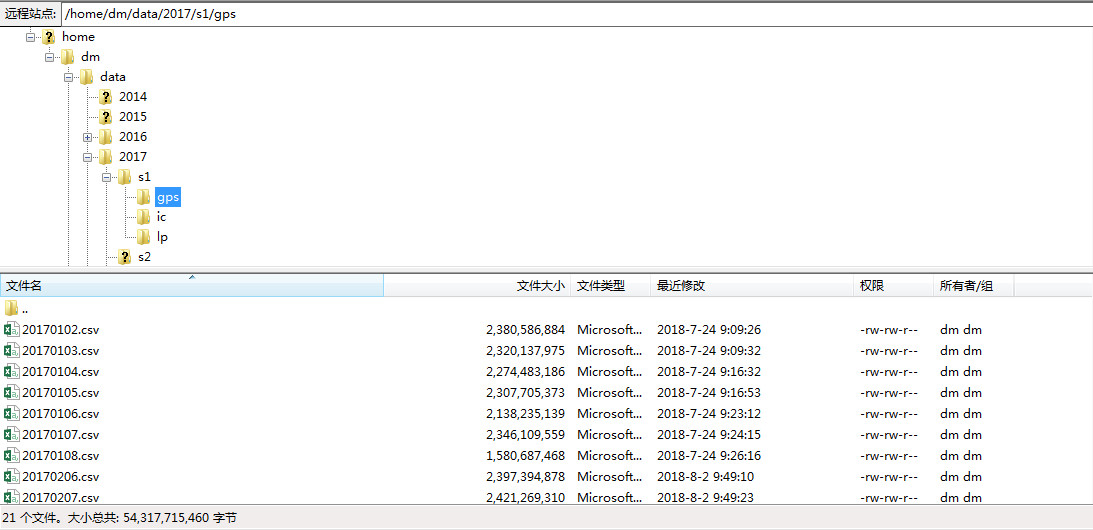
\includegraphics[width=\textwidth]{figures/chp02_分类集中存储后的目录结构.jpg}
  \caption{分类集中存储后的目录结构\label{fig:分类集中存储后的目录结构}} 
%\end{center}   
\end{figure}

\section{静态 GIS 数据处理} \label{sec:静态GIS数据处理}
静态 GIS 数据指用于展示和分析的 GIS 图层数据, 包括各类区域边界、 道
路网络、公交网络站点的形状和属性信息等, 主要用于制作各类交通专题图、基
础统计以及辅助数据挖掘计算。 其变化频率低、 更新周期较长,一般为一年更新
一次,因此相对于动态交通数据的高更新频率来说属于静态数据。

\subsection{现有数据类型} \label{sec:现有数据类型}
深圳市交通仿真系统(二期) 中囊括的静态 GIS 数据包括: 基础 GIS 数据
(行政区、水系、绿地、法定图则、组团、街道),基层路网数据(道路节点、
路段、交通小区、主要节点数据),公交和轨道 GIS 数据(公交站点、公交网络、
轨道站点、轨道网络),调查数据(居民出行调查、轨道二期开通后调查、交叉
口/断面流量调查等),现状和规划土地利用(建筑物普查数据、规划一张图),
现状和规划人口岗位数据, POI 数据(医院、学校、口岸、火车站、飞机场、港
口、公共停车场、 检测器), 共 4 大类 26 小类。详细表信息见附表。

其中, 道路数据和公交数据涉及后续的数据挖掘系统输入,需要进行年度更
新,其他 GIS 数据根据需求不定期进行更新。 为了提高工作效率, 数据更新工
作按照不同 GIS 图层并行开展, 更新后的 GIS 数据以 shapefile 格式进行存储,
待后续数据挖掘和数据查询系统使用。

\subsection{道路数据更新}
道路数据更新的技术方法是:以市规划国土委(海洋局)信息中心提供的最
新版深圳市道路网络数据为底图,按照交通模型和查询的数据结构需求,采用
ArcGIS 软件在深圳市交通仿真系统(二期)已有的 \ppyear 年路网图层(Roadlink)
和节点图层(RoadNode)基础上,进行全人工道路形状和属性编辑,将现状道路
数据更新至 \pyear 年 12 月。

更新的流程包括更新道路形状、更新道路节点、更新道路属性、质量检查和
更新数据挖掘专用道路数据五个环节(见\fref{fig:道路数据更新流程})

\begin{figure}[ht]
  \centering
  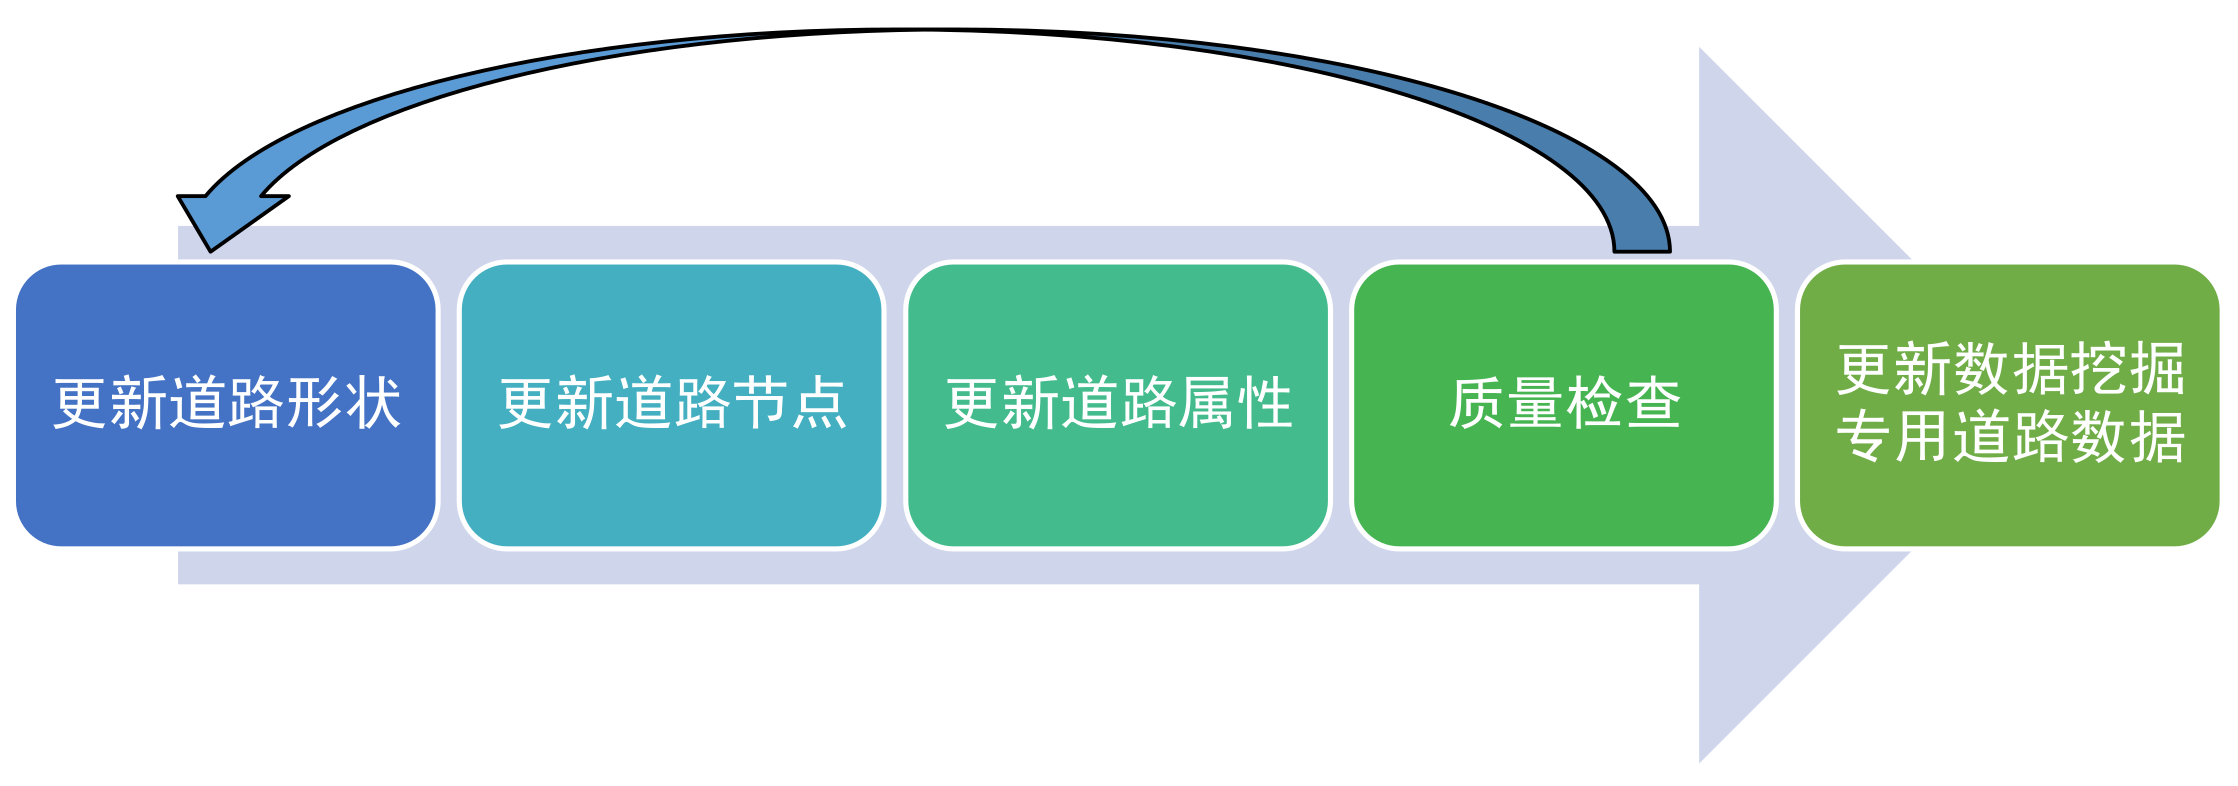
\includegraphics[width=\textwidth]{figures/chp02_道路数据更新流程.png}
  \caption{道路数据更新流程\label{fig:道路数据更新流程} }
\end{figure}

\subsubsection{更新道路形状}
道路形状更新有三种情况:新增路段、删除路段和修改路段。

\smalltitle{新增路段}
新增路段在年度更新中出现的情况最多,主要工作是把年度新增的道路在
GIS 数据中进行更新,包括以下三种场景:

\begin{nbeae}
\item 在两个已有节点之间增加路段\\
\indenttext{在两条道路的交叉口之间新修道路时适用此情况。}

\indtentext{操作步骤:打开 ArcMap 的节点捕捉功能,先选择其中一个已有节点;然后
再根据信息中心底图数据的形状绘制新增路段,直至另一个已有节点;最后结束
形状编辑操作。}

\indenttext{如下图所示,在 16258 节点和 16362 节点之间新增路段。}

\begin{figure}[ht]
  \centering
  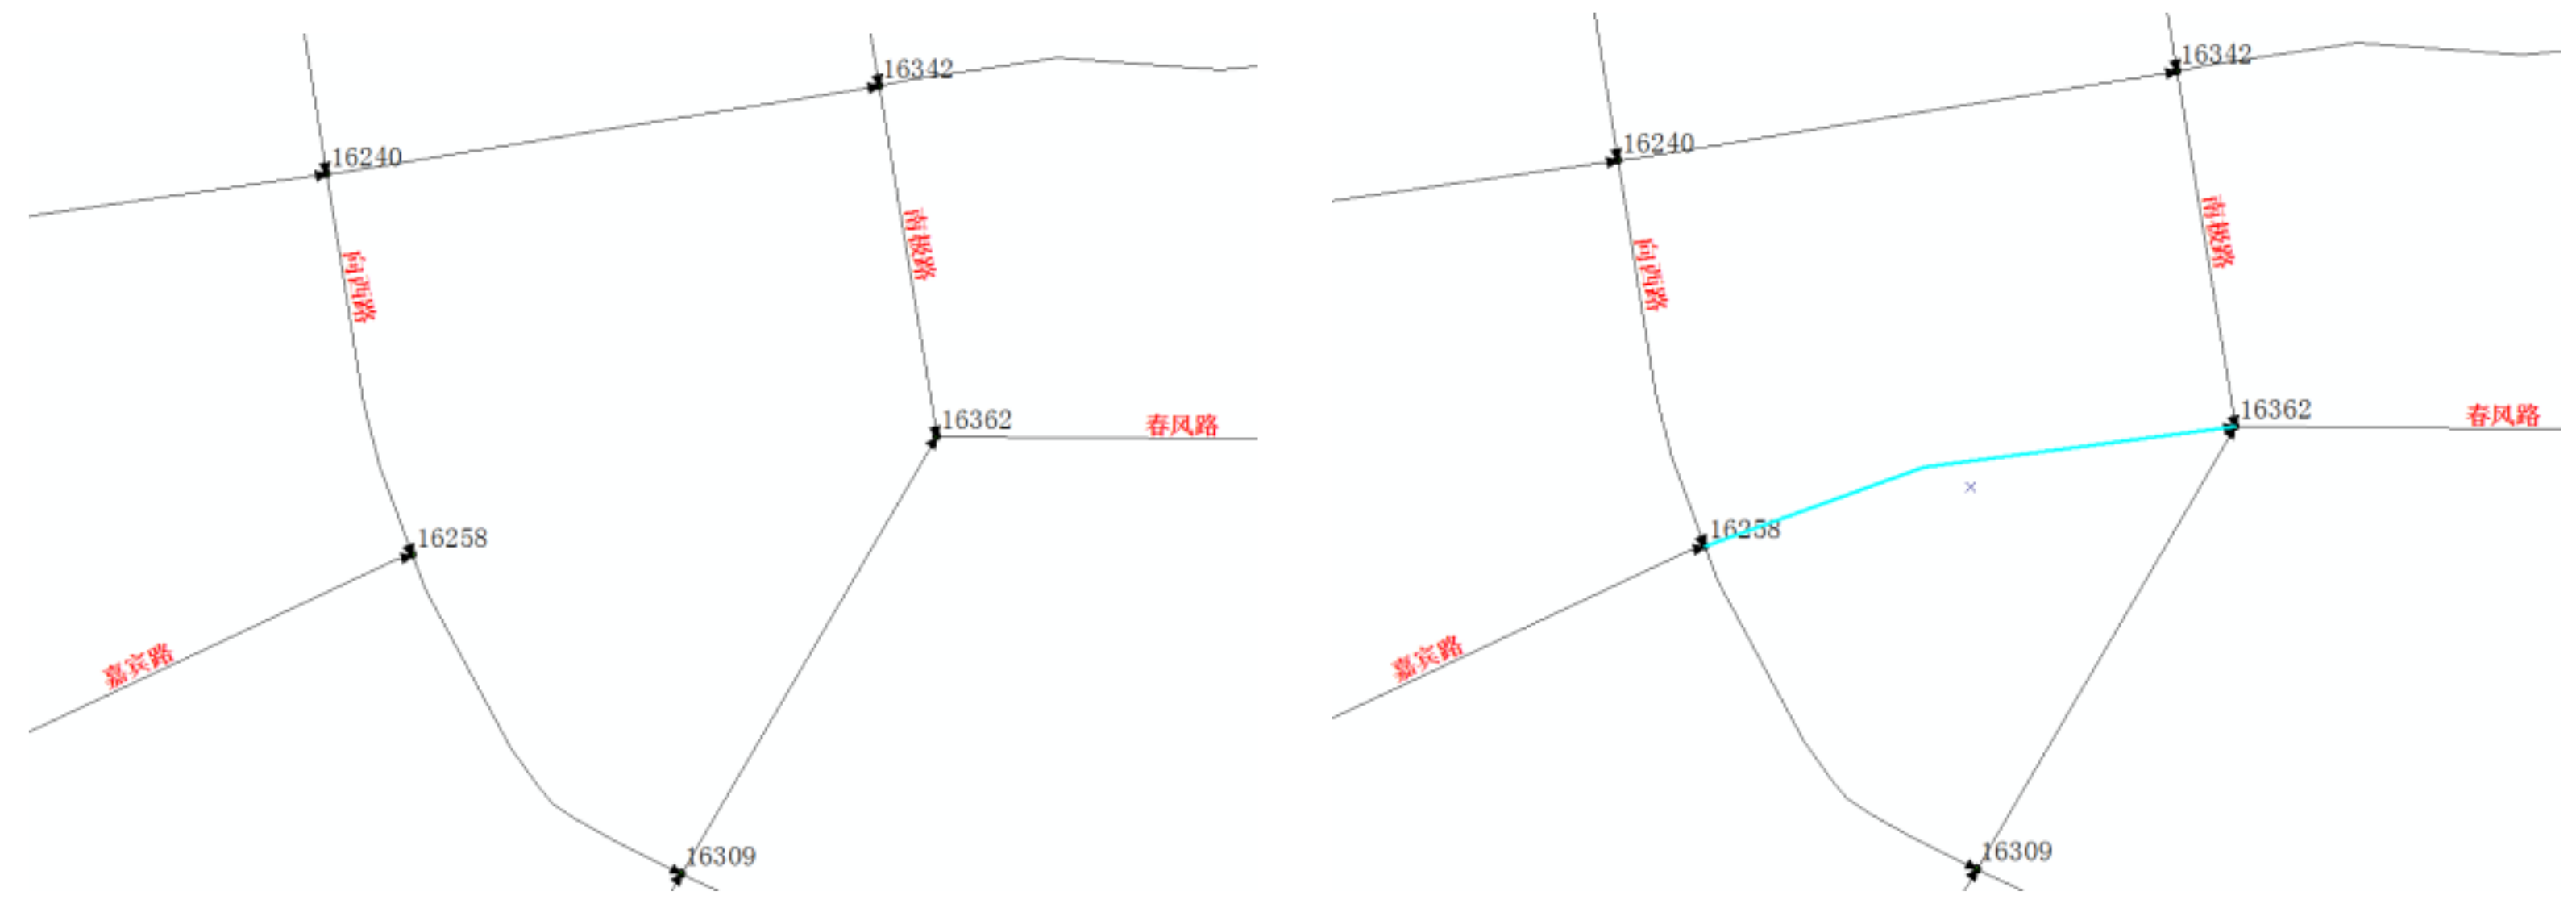
\includegraphics[width=\textwidth]{figures/chp02_在已知两个节点之间增加路段.png}
  \caption{在已知两个节点之间增加路段\label{fig:在已知两个节点之间增加路段} }
\end{figure}

\item 在一个已有节点和一个新增节点之间增加路段\\
\indenttext{在一条道路的交叉口与另一条道路新增交叉口之间新修道路时适用此情况。}

\indenttext{操作步骤:首先根据信息中心底图数据的形状,将已有路段打断;然后在打
断的位置处新增一个节点,最后按照(a)的步骤在已有节点和新增节点绘制新增路段。}

\begin{figure}[ht]
  \centering
  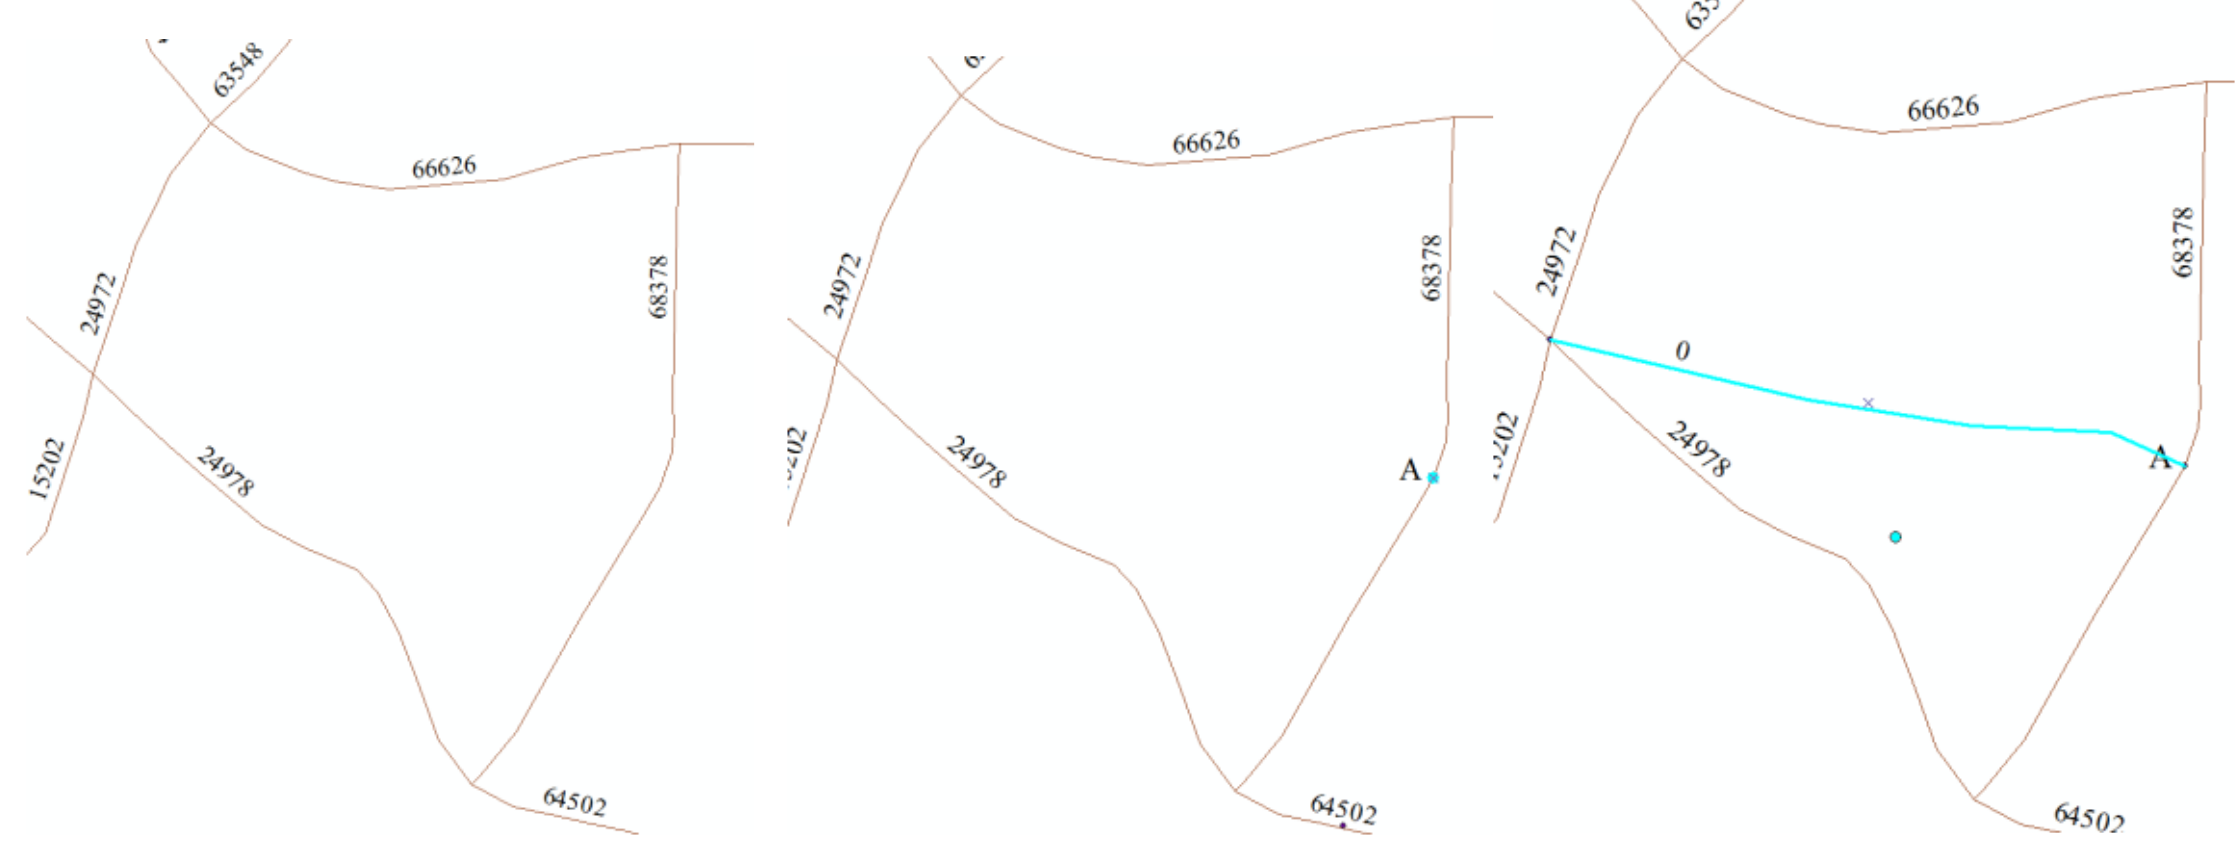
\includegraphics[width=\textwidth]{figures/chp02_在一个已有节点和一个新增节点之间增加路段.png}
  \caption{在一个已有节点和一个新增节点之间增加路段\label{fig:在一个已有节点和一个新增节点之间增加路段} }
\end{figure}

\item 在两个新增节点之间增加路段\\
\indenttext{在两个新增节点之间增加路段的情况较少出现,适用于在两条道路都新增的交叉口之间新修道路的场景。
操作步骤与(1)类似,但是需要在两条道路上都先做打断和新增节点操作。}
\end{nbeae}

\smalltitle{删除路段}
删除路段用于原先绘制的道路错误、道路废弃等情况,一般较少出现。

操作步骤:首先选中需要删除的路段,然后点击删除指令,最后结束编辑。

\smalltitle{修改路段}
修改路段主要用于道路大致位置不变,即首尾节点不变的情况下,原绘制的
路段形状与实际情况存在较大差异时,需要对道路的形状进行修正。修改路段形
状对于道路原有的连接关系没有影响,不会影响交通仿真模型的运算结果,但是
会影响数据挖掘中 GPS 数据地图匹配的精度。

操作步骤:选择待修改路段,打开节点编辑功能,按照信息中心底图进行形
状修改,最后结束编辑。

\subsubsection{更新道路节点}
道路节点的更新主要是在道路形状发生改变的路段基础上,新增相应的道路
节点,用于表示道路交叉口;另外,还会对原有的道路节点进行删除和修改等修
复性工作。按照深圳市交通仿真系统(二期)的数据需求,在所有会发生行驶转
向的交叉口都需要有相应的节点数据,而其他情况的节点都不需要保存。

操作步骤:打开捕捉节点功能,按照实际的道路交叉口进行新增节点、删除
节点和修改节点的操作,最后结束编辑。

更新道路节点的工作需要特别注意是高架桥和隧道等区域,在这些区域由于
道路与道路是立体交叉的,并不会产生行驶转向,因此不能仅通过图形判断,必
须进行实地踏勘或者从卫星影像图中获得实际的转向信息。

\subsubsection{更新道路属性}
上述两个步骤完成了道路的基本形状:路段和节点的更新,但是道路是具有
特殊交通属性的线状实体,因此要在形状更新的基础上进一步更新道路的交通属
性信息,用于描述真实的道路。道路的属性更新工作可以和形状更新同步开展,
也可以在形状更新之后批量修改,所有的操作都由人工完成。

深圳市交通仿真系统(二期)中构建的路段图层 Roadlink 和节点图层
RodeNode 的属性信息见附录。

路段图层包含的属性信息非常多,其中必须要更新的为路段唯一 ID 字段,
起止节点编号字段,路段长度字段,起节点向终节点方向和终节点向起节点方向
字段,道路等级字段,所在行政区、所在交通小区、所在街道、所在组团、所在
法定图则、所属吸引点字段。

其中,新增加路段的 NO 值,在原有最大 NO 值的基础上增加 1 或 2,如为
单行线,则为 1,如为双行线,则为 2;如果删除路段,原有的 NO 值不再使用,
修改路段不需要修改原有 NO 值。路段长度、起节点向终节点方向和终节点向起
节点方向、所在行政区、所在交通小区、所在街道、所在组团、所在法定图则、
所属吸引点字段可以在形状更新完成后通过 ArcGIS 自带的数据处理工具自动化
辅助更新。

节点图层必须要更新的字段是唯一 ID 和坐标 X、坐标 Y。其中,新增加节
点的 WYID 值,在原有最大 WYID 值的基础上增加 1;坐标 X 和坐标 Y 可以在
形状更新完成后通过 ArcGIS 自带的数据处理工具自动化辅助更新。

\subsubsection{质量检查}
由于上述的操作主要由人工完成,所以在操作过程中难免会出现一些错误,
因此需要通过预设的一些规则自动筛选出可能出现错误的地方,然后再通过人工
判断确定错误的位置,最后按照上述形状和属性更新的步骤来修复错误。为了保
证数据的质量,质量检查工作同时由多人配合完成。

数据质量检查包括操作过程中的日志记录和后期的自动化检查两部分。其中
日志记录是今年新引入的一种工作模式,其原理是在每一步操作中记录操作内容
和操作时间,目的是为了能够在后期检查中发现错误操作时能够进行有效的回退
操作,减少人工排查的工作量并提高修复精度。

自动化检查部分包括:路段 ID 的唯一性检查、小路段的检测与修复、断头路的检测与修复、
相连相同路段的检测与修复以及道路立体交叉处的连接关系修复。

\smalltitle{路段 ID 的唯一性检查}
路段的 ID 是后续数据挖掘和数据查询的重要条件,如果在人工作业中出现
了重复 ID,则会导致后续挖掘和数据查询的错误结果,因此需要通过程序自动
化检查路段 ID 是否出现重复。

\smalltitle{小路段的检测与修复}
小路段是指路段长度小于一定阈值的路段。小路段的存在大大增加了系统负
荷,降低了系统执行效率。因此,本项目以 50 米为阈值,对全路网进行检测,
并人工编辑修复 50 米以下路段。

\begin{figure}[ht]
  \centering
  
\includegraphics[width=0.6\textwidth]{figures/chp02_小路段的检测与修复.png}
  \caption{小路段的检测与修复\label{fig:小路段的检测与修复}}
\end{figure}

\smalltitle{断头路的检测与修复}
断头路是指路段到了终点后,没有后续相连的道路与之连接。断头路分为正
常断头路和非正常断头路。非正常断头路事实上是拓扑逻辑存在问题的区域,因
此必须予以消除。

\begin{figure}[ht]
  \centering
  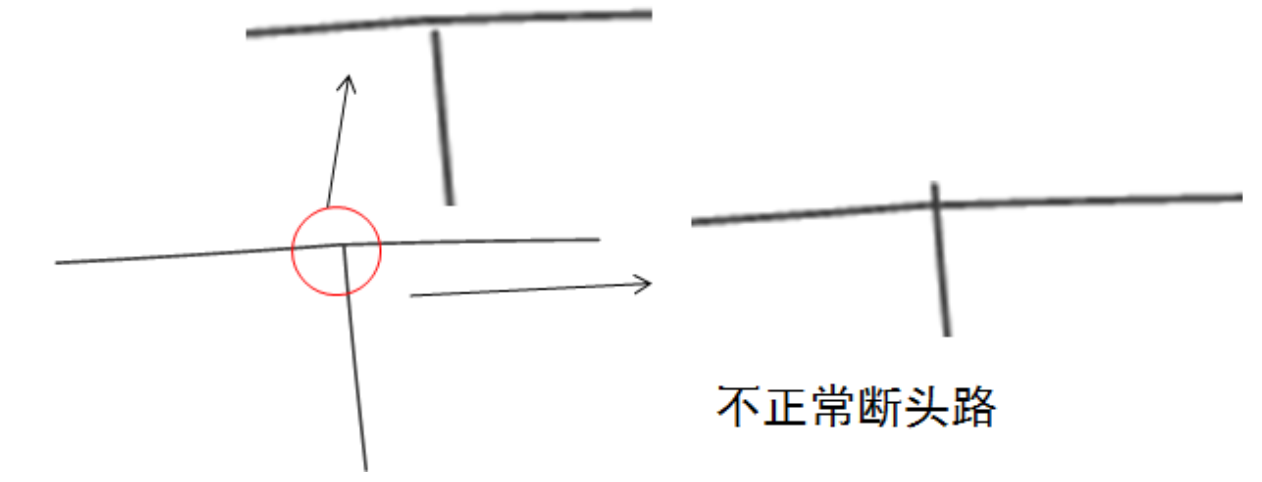
\includegraphics[width=0.6\textwidth]{figures/chp02_断头路的检测与修复.png}
  \caption{断头路的检测与修复\label{fig:断头路的检测与修复}}
\end{figure}

\smalltitle{相连相同路段的检测与修复}
相连相同路段是指道路名称(DLMC)、车道数(CDS)、道路等级(DLDJ)、
分割类型(CGLX)等四个关键属性完全一致的道路,这种类型的道路事实上可
以进行合并管理

\begin{figure}[!ht]
  \centering
  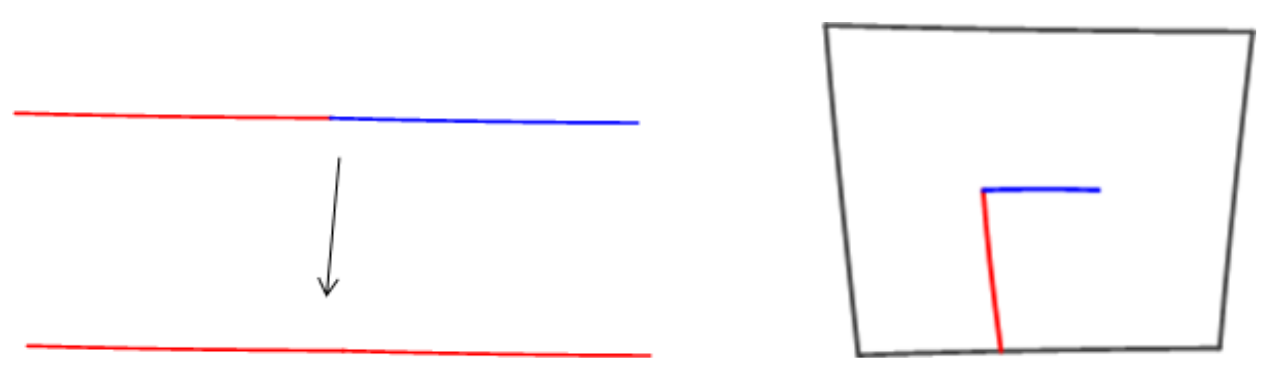
\includegraphics[width=0.6\textwidth]{figures/chp02_相连相同路段的检测与修复.png}
  \caption{相连相同路段的检测与修复\label{fig:相连相同路段的检测与修复}}
\end{figure}

\smalltitle{道路立体交叉处的连接关系修复}
对于匝道、立交桥、隧道等立体交叉位置,采用卫星影像辅助人工判断道路的实际连接关系。

\begin{figure}[!ht]
  \centering
  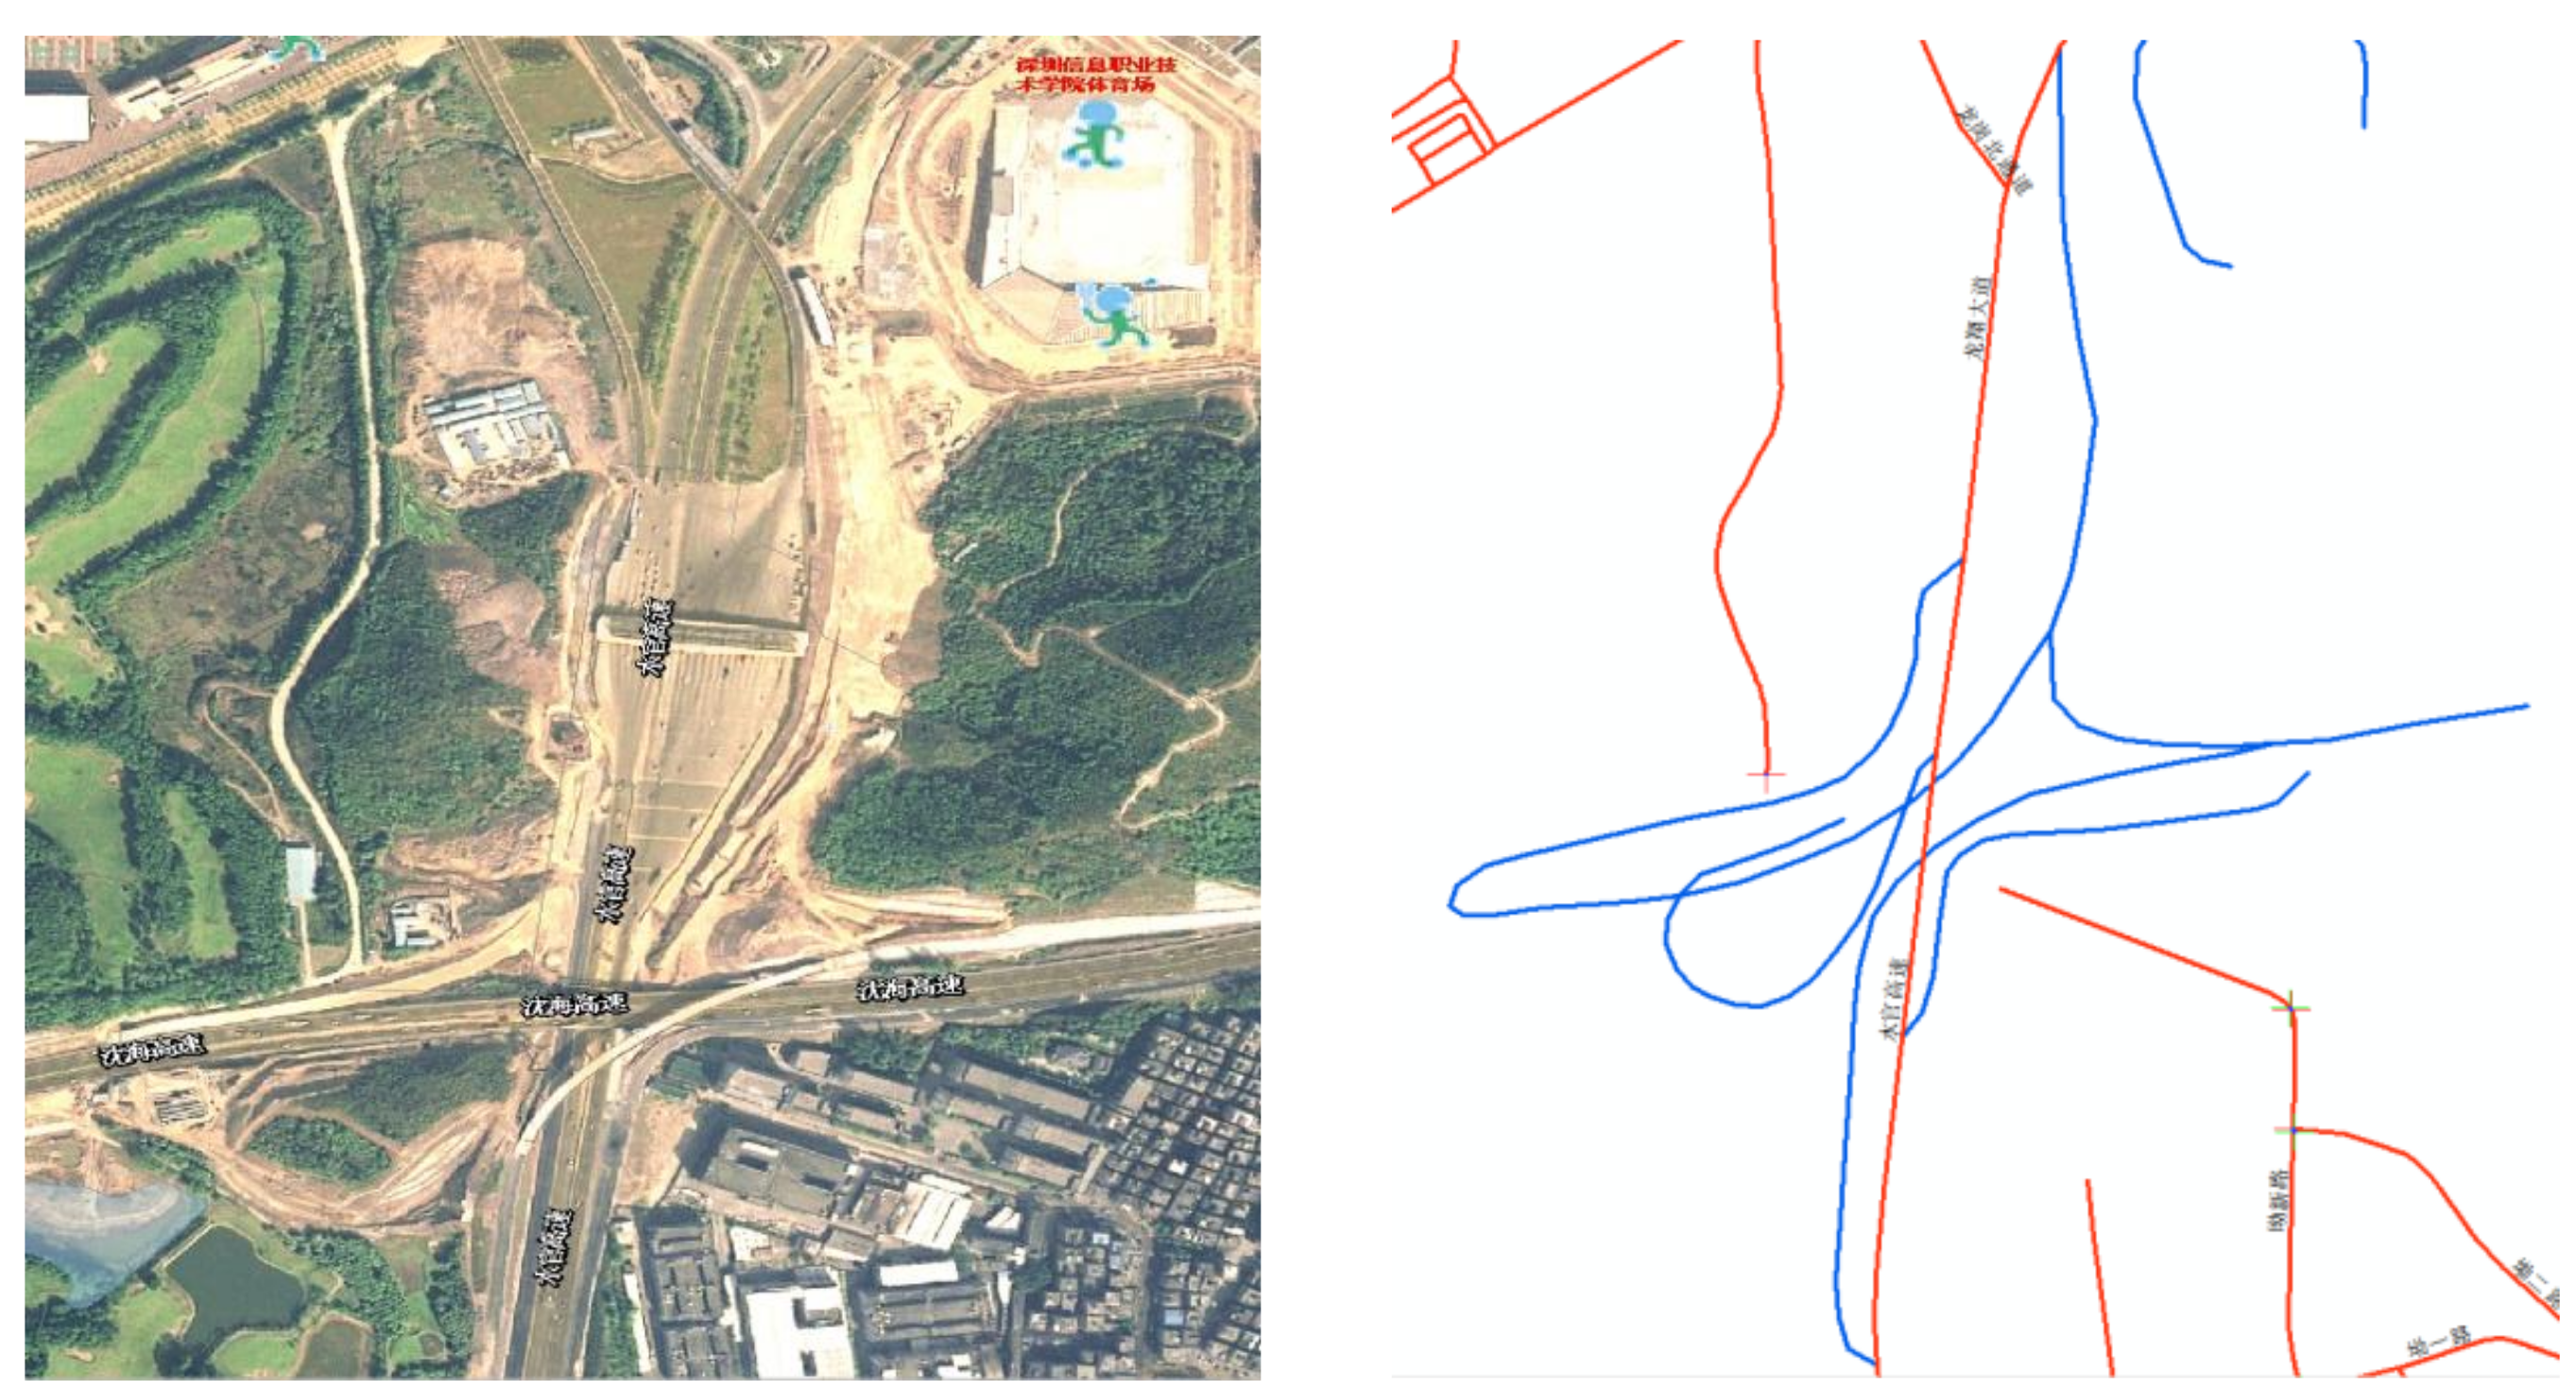
\includegraphics[width=0.6\textwidth]{figures/chp02_道路立体交叉处的连接关系修复.png}
  \caption{道路立体交叉处的连接关系修复\label{fig:道路立体交叉处的连接关系修复}}
\end{figure}

\subsubsection{公交数据更新}
公交数据更新的技术方法是:基于交委发布的现状公交站点名称数据,并结
合商业地图中的现状公交站点位置数据,以深圳市交通仿真系统(二期)原有的
公交站点图层(BusStop)为基础,采用半自动化方式进行新增和修改操作;然
后再通过专门开发的程序,按照站点位置和线路站点顺序,重新生成公交线路,
直接更换原有数据。

更新的流程包括更新公交站点位置和名称、公交网检查、生成公交线路和更
新线路和站点属性四个环节。

\begin{figure}[ht]
  \centering
  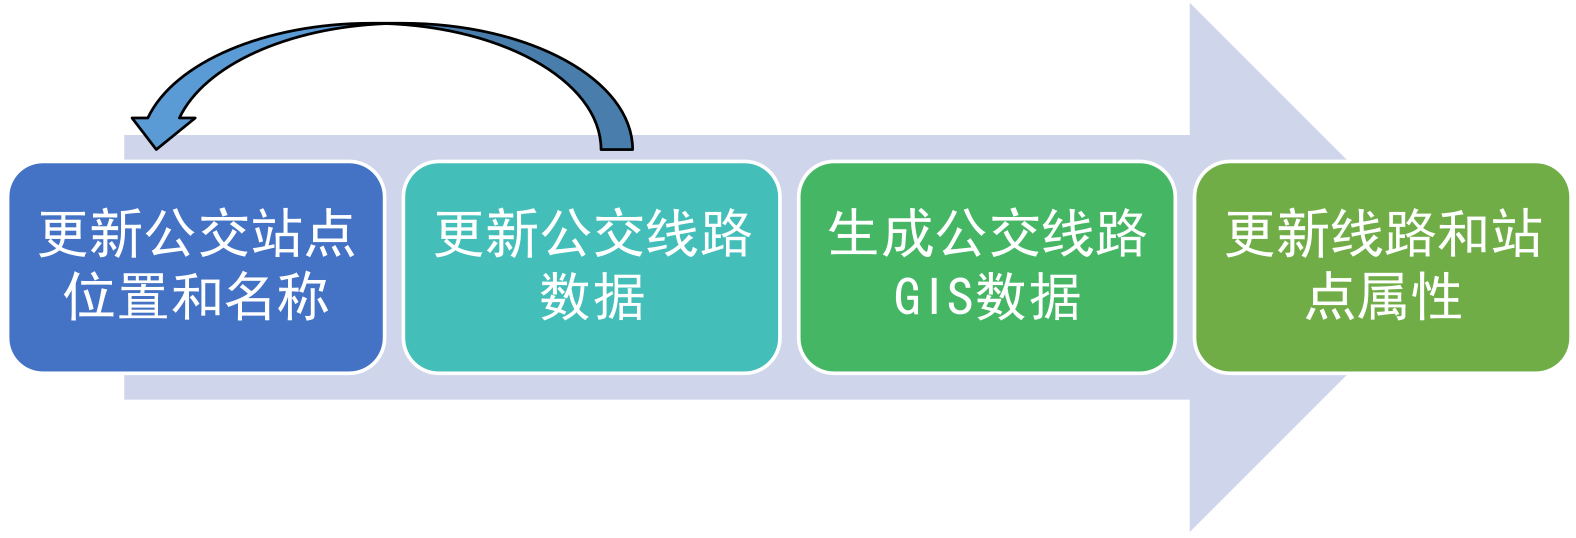
\includegraphics[width=\textwidth]{figures/chp02_公交数据更新流程.png}
  \caption{公交数据更新流程\label{fig:公交数据更新流程} }
\end{figure}


\subsubsection{其他 GIS 数据更新}
根据 \ref{sec:现有数据类型}节显示的深圳市交通仿真系统(二期)所有静态 GIS 数据,除了
需要进行年度更新的道路数据和公交数据之外,其他的 GIS 数据可以根据年度
的实际情况进行更新,更新的范围也包括图形和属性更新两部分。例如,某些区
域图层的边界发生变化,或者新开通了轨道线路和站点等情况。
2016 年由于交警新增了一部分车牌识别监测点,因此本项目也同步更新了
点位的 GIS 图层(Detector)。其主要属性见附录。

\section{年度更新成果}
\subsection{动态交通数据}
按照\ref{sec:动态交通数据处理}节进行预处理后的动态交通数据,通过 FTP 方式上传到数据挖掘主
机上,按照\ref{subsec:分类集中存储}节的文件夹结构进行统一存储,下面列出更新后的文件
夹包含文件的信息。

\begin{table}[htpb]\centering 
  \caption{更新后的公交GPS数据成果\label{tbl:更新后的公交GPS数据成果}}
%\subfloat[公交 GPS 数据]  
\begin{tabularx}{\textwidth}{|c|X|}
    \hline
    \multirow{4}*{\centering 路径} & 第一季度:/home/dm/data/\pyear /s1/gps\\
    & 第二季度:/home/dm/data/\pyear /s2/gps \\
    & 第三季度:/home/dm/data/\pyear /s3/gps \\
    & 第四季度:/home/dm/data/\pyear /s4/gps \\\hline
    文件名 & 日期.csv,如 \pyear 0101.csv,共 84 个\\\hline
    说明 & 标准化预处理并以日为单位合并后的公交 GPS 数据,每天一个文件存储 \\\hline
    大小 & \\
    \hline
  \end{tabularx}
\end{table}
%\subfloat[深圳通 IC 刷卡数据] 
\begin{table}[htpb]\centering
\caption{更新后的深圳通刷卡数据成果\label{tbl:更新后的深圳通刷卡数据成果}} 
\renewcommand\tabularxcolumn[1]{m{#1}}
\begin{tabularx}{\textwidth}{|c|X|}
    \hline
    \multirow{4}*{路径} & 第一季度:/home/dm/data/\pyear /s1/ic\\
    & 第二季度:/home/dm/data/\pyear /s2/ic \\
    & 第三季度:/home/dm/data/\pyear /s3/ic \\
    & 第四季度:/home/dm/data/\pyear /s4/ic \\\hline
    文件名 & ic\_bus\_月份.csv(公交刷卡数据)、 ic\_metro\_月份.csv(轨道刷卡数据),如ic\_bus\_01.csv、ic\_metro\_12.csv,共24个\\\hline
    说明 & 标准化预处理并以日为单位合并后的公交 GPS 数据,每天一个文件存储 \\\hline
    大小 & \\
    \hline
  \end{tabularx}
\end{table}

%\ContinuedFloat
%\subfloat[车牌识别数据]
\begin{longtabu} to \textwidth{|c|X[1,l]|}
\caption{更新后的车牌识别数据成果\label{tbl:更新后的车牌识别数据成果}} 
  \hline
  \multirow{4}*{路径} & 第一季度:/home/dm/data/\pyear /s1/lp\\
    & 第二季度:/home/dm/data/\pyear /s2/lp \\
    & 第三季度:/home/dm/data/\pyear /s3/lp \\
    & 第四季度:/home/dm/data/\pyear /s4/lp \\\hline
    文件名 & sbbak+日期.txt,如 sbbak\pyear -01-06.txt,共84个\\\hline
    说明 & 标准化预处理并以日为单位合并后的车牌识别数据,每天一个文件存储 \\\hline
    大小 & \\
    \hline
\end{longtabu}
%\end{table}


% \begin{table}[htpb]\centering 
%   \caption{更新后的动态交通数据成果\label{tbl:更新后的动态交通数据成果}}
% \subfloat[第一季度公交 GPS 数据(每天一个文件存储)]  
% {\begin{tabularx}{\textwidth}{|c|X|}
%     \hline
%     路径 & /home/dm/data/\pyear /s1/gps\\\hline
%     文件名 & 日期.csv,如 \pyear 0101.csv,共 21 个\\\hline
%     说明 & 标准化预处理并以日为单位合并后的公交 GPS 数据 \\\hline
%     大小 & \\
%     \hline
%   \end{tabularx}}\\
% \subfloat[第一季度深圳通 IC 刷卡数据]
% {\begin{tabularx}{\textwidth}{|c|X|}
%     \hline
%     路径 & /home/dm/data/\pyear /s1/ic\\\hline
%     文件名 & ic\_bus\_01.csv、 ic\_bus\_02.csv、 ic\_bus\_03.csv、 ic\_metro\_01.csv、 ic\_metro\_02.csv、
% ic\_metro\_03.csv\\\hline
%     说明 & 公交和轨道深圳通 IC 刷卡数据 \\\hline
%     大小 & \\
%     \hline
%   \end{tabularx}}\\
% \subfloat[第一季度车牌识别数据]
% {\begin{tabularx}{\textwidth}{|c|X|}
%     \hline
%     路径 & /home/dm/data/\pyear /s1/lp\\\hline
%     文件名 & sbbak+日期.txt,共 21 个,如 sbbak \pyear -01-06.txt\\\hline
%     说明 & 公交和轨道深圳通 IC 刷卡数据 \\\hline
%     大小 & \\
%     \hline
%   \end{tabularx}}\\
% \subfloat[第二季度公交 GPS 数据(每天一个文件存储)]  
% {\begin{tabularx}{\textwidth}{|c|X|}
%     \hline
%     路径 & /home/dm/data/\pyear /s2/gps\\\hline
%     文件名 & 日期.csv,如 \pyear 0101.csv,共 21 个\\\hline
%     说明 & 标准化预处理并以日为单位合并后的公交 GPS 数据 \\\hline
%     大小 & \\
%     \hline
%   \end{tabularx}}\\
% \end{table}

% \begin{table}[htpb]\centering 
% \ContinuedFloat
% \subfloat[第二季度深圳通 IC 刷卡数据]
% {\begin{tabularx}{\textwidth}{|c|X|}
%     \hline
%     路径 & /home/dm/data/\pyear /s2/ic\\\hline
%     文件名 & ic\_bus\_04.csv、 ic\_bus\_05.csv、 ic\_bus\_06.csv、 ic\_metro\_04.csv、 ic\_metro\_05.csv、
% ic\_metro\_06.csv\\\hline
%     说明 & 公交和轨道深圳通 IC 刷卡数据 \\\hline
%     大小 & \\
%     \hline
%   \end{tabularx}}\\
% \subfloat[第二季度车牌识别数据]
% {\begin{tabularx}{\textwidth}{|c|X|}
%     \hline
%     路径 & /home/dm/data/\pyear /s2/lp\\\hline
%     文件名 & sbbak+日期.txt,共 21 个,如 sbbak \pyear -01-06.txt\\\hline
%     说明 & 公交和轨道深圳通 IC 刷卡数据 \\\hline
%     大小 & \\
%     \hline
%   \end{tabularx}}\\ 
% \subfloat[第三季度公交 GPS 数据(每天一个文件存储)]  
% {\begin{tabularx}{\textwidth}{|c|X|}
%     \hline
%     路径 & /home/dm/data/\pyear /s3/gps\\\hline
%     文件名 & 日期.csv,如 \pyear 0101.csv,共 21 个\\\hline
%     说明 & 标准化预处理并以日为单位合并后的公交 GPS 数据 \\\hline
%     大小 & \\
%     \hline
%   \end{tabularx}}\\
% \subfloat[第三季度深圳通 IC 刷卡数据]
% {\begin{tabularx}{\textwidth}{|c|X|}
%     \hline
%     路径 & /home/dm/data/\pyear /s3/ic\\\hline
%     文件名 & ic\_bus\_07.csv、 ic\_bus\_08.csv、 ic\_bus\_09.csv、 ic\_metro\_07.csv、 ic\_metro\_08.csv、
% ic\_metro\_09.csv\\\hline
%     说明 & 公交和轨道深圳通 IC 刷卡数据 \\\hline
%     大小 & \\
%     \hline
%   \end{tabularx}}\\
% \subfloat[第三季度车牌识别数据]
% {\begin{tabularx}{\textwidth}{|c|X|}
%     \hline
%     路径 & /home/dm/data/\pyear /s3/lp\\\hline
%     文件名 & sbbak+日期.txt,共 21 个,如 sbbak \pyear -01-06.txt\\\hline
%     说明 & 公交和轨道深圳通 IC 刷卡数据 \\\hline
%     大小 & \\
%     \hline
%   \end{tabularx}}\\
% \subfloat[第四季度公交 GPS 数据(每天一个文件存储)]  
% {\begin{tabularx}{\textwidth}{|c|X|}
%     \hline
%     路径 & /home/dm/data/\pyear /s4/gps\\\hline
%     文件名 & 日期.csv,如 \pyear 0101.csv,共 21 个\\\hline
%     说明 & 标准化预处理并以日为单位合并后的公交 GPS 数据 \\\hline
%     大小 & \\
%     \hline
%   \end{tabularx}}\\
% \end{table}

% \begin{table}[htpb]\centering 
%   %\caption{更新后的动态交通数据成果\label{tbl:更新后的动态交通数据成果}}
% \ContinuedFloat
% \subfloat[第四季度深圳通 IC 刷卡数据]
% {\begin{tabularx}{\textwidth}{|c|X|}
%     \hline
%     路径 & /home/dm/data/\pyear /s4/ic\\\hline
%     文件名 & ic\_bus\_10.csv、 ic\_bus\_11.csv、 ic\_bus\_12.csv、 ic\_metro\_10.csv、 ic\_metro\_11.csv、
% ic\_metro\_12.csv\\\hline
%     说明 & 公交和轨道深圳通 IC 刷卡数据 \\\hline
%     大小 & \\
%     \hline
%   \end{tabularx}}\\
% \subfloat[第四季度车牌识别数据]
% {\begin{tabularx}{\textwidth}{|c|X|}
%     \hline
%     路径 & /home/dm/data/\pyear /s4/lp\\\hline
%     文件名 & sbbak+日期.txt,共 21 个,如 sbbak \pyear -01-06.txt\\\hline
%     说明 & 公交和轨道深圳通 IC 刷卡数据 \\\hline
%     大小 & \\
%     \hline
%   \end{tabularx}}\\
% \end{table}

%\afterpage{\clearpage}
\subsection{静态 GIS 数据}
更新前的深圳市交通仿真系统(二期)道路 GIS 数据共有 39396 条路段,
本年度更新的道路 GIS 数据包括:新增建设完成的前海片区、龙华新区等市内
主要道路,修正和合并部分次干路和支路并删除部分支路和小区道路,更新后共
有 40142 条路段,更新路段数量为 1105 条,道路节点 504 个。下图为年度更新
道路 GIS 数据的空间分布情况。

\subsection{公交GIS数据}
% \begin{longtabu} to \textwidth {|X[1,c]|X[1,c]|X[1,c]|X[1.2,c]|X[1.2,c]|}
% \caption{现有静态 GIS 数据\label{tbl:现有静态 GIS 数据}} 
%   \hline
%   \multicolumn{1}{|c|}{\bfseries 类别} & \multicolumn{1}{c|}{\bfseries 名称} &
%   \multicolumn{1}{c|}{\bfseries 格式} & \multicolumn{1}{c|}{\bfseries 主要属性} &
%   \multicolumn{1}{c|}{\bfseries 更新周期} \\\hline
%    & 行政区 & shapefile & 名称、 关内关外 & 由信息中心提供\\\hline
%   \multirow{6}*{基础GIS数据} & 水系 & shapefile & 名称 & 由信息中心提供\\\cline{2-5}
%    & 绿地 & shapefile & 名称 & 由信息中心提供\\\cline{2-5}
%    & 法定图则 & shapefile & 名称 & 由信息中心提供\\\cline{2-5}
%    & 组团 & shapefile & 名称 & 由信息中心提供\\\cline{2-5}
%    & 街道 & shapefile & 名称 & 由信息中心提供\\\cline{2-5}
%    & 人口普查小区 & shapefile & 名称 & 由信息中心提供\\\hline
%    \multirow{5}*{基础路网数据} & 现状道路节点 & shapefile & 坐标、节点类型、所在行政区、所在交通小区、所在街
% 道、所在组团、所在法定图则、交叉口控制类型、立交类型 & 由信息中心提供\\\cline{2-5}
%    & 主要交叉口 & shapefile & 同上 & 不定期  \\\cline{2-5}
%    & 现状道路网络 & shapefile & 起止节点编号、起止道路名称、道路
% 名称、车道数、长度、宽度、机动车道宽度、非机动车道宽度、人行道宽度、 机非分隔带宽
% 度、 中央分隔带宽度、 红线宽度、 道路等级、行车方向、建设方式、 分割类型、 是否具备公交
% 专用道、 交通系统集、 设计车速、 路段通行能力、 路段延误函数、 所在行政区、 所在交通小
% 区、 所在街道、 所在组团、 所在法定图则、 最后更新时间 & 年度 \\\cline{2-5}
%    & 规划道路网络 & shapefile & 同上 & 不定期 \\\cline{2-5}
%    & 交通小区 & shapefile & 形心坐标、所在行政区、所在街道、所在组团、所在法定图则 & 不定期\\\cline{2-5}
% \hline
% \end{longtabu}

